\section{Arquitectura de Software}

Basándose en los estudios preliminares, tanto del informe de requerimientos,
protocolos y estándares de IVOA, y considerando los requerimientos expuestos y
sus respectivos casos de uso, se tomó la decisión de crear una arquitectura de
tres capas, la cual se expone en el siguiente diagrama:
\vspace{1.0cm}
\begin{figure}[h!t]
    \begin{center}
        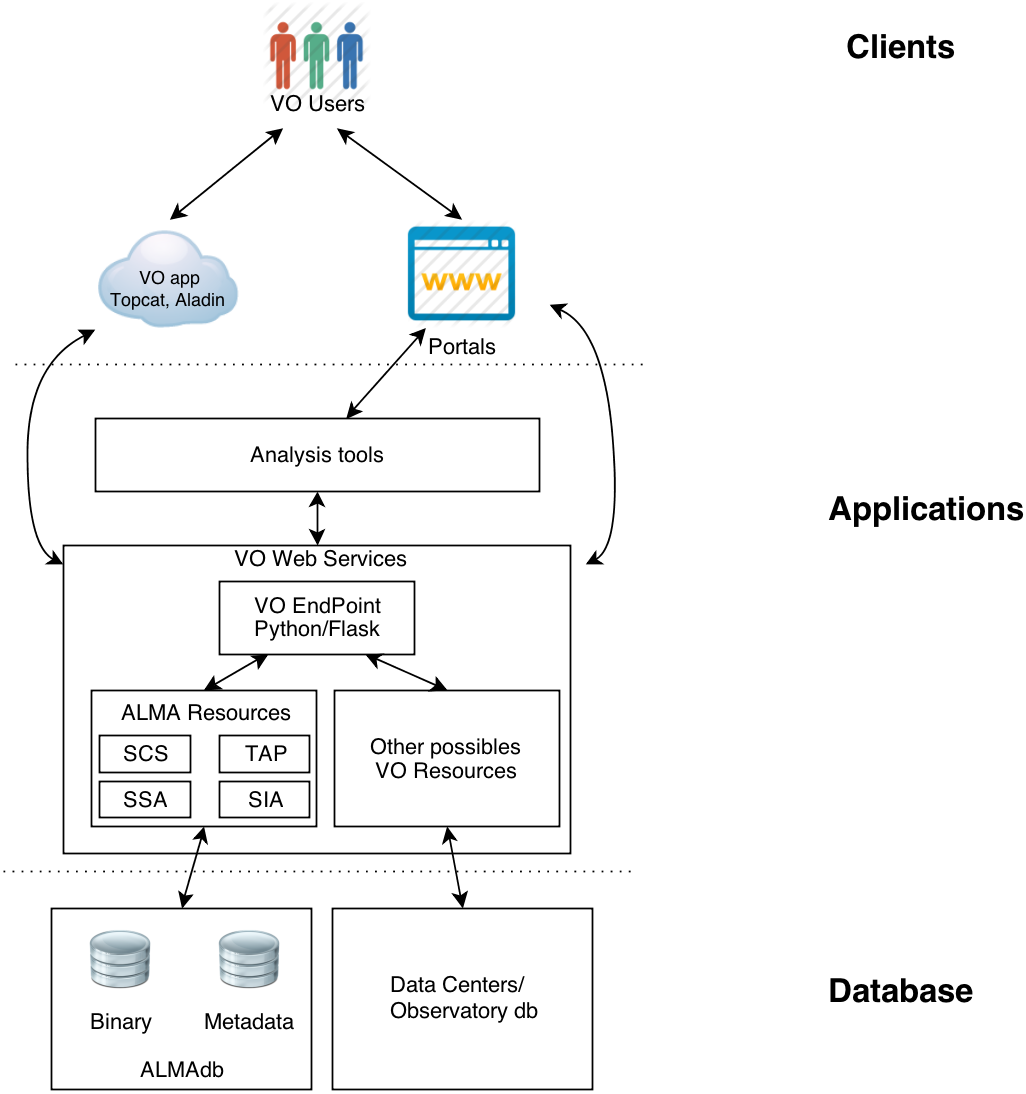
\includegraphics[width=0.6\textwidth]{img/chivo_capas.png}
        \caption{Arquitectura ChiVO - Tres capas.}
    \end{center}
\end{figure}

\subsection{Capa de Datos}
En esa capa residen los datos y es la encargada de organizar estos en una
estructura apropiada. Se implementó una base de datos relacional usando el
motor de base de datos postgresql \cite{psql} y el modelo de datos a usar es
ObsCore \cite{obscore}.

IVOA recomienda usar el modelo de datos ObsCore como base para su
interoperabilidad, definiendo columnas y tipos de datos conocidos de tal manera
que sea sencillo acceder y descrubrir información dentro de la base de datos.
Por otro lado todos los toolkits estudiados que soportan los Data Access Layer
en IVOA usan una función de postgresql llamada pgSphere \cite{pgsphere}. Estas
fueron las consideraciones para elegir dichas tecnologías.

Como los datos públicos del ciclo 0 de ALMA estarán todos disponibles en Abril
del 2014, en este prototipo se probó la interacción entre la capa de datos con
aplicación con datos de prueba. Una vez que todos estos datos estén disponibles
se poblará con datos reales la base de datos.

\subsection{Capa de Aplicación}
En la capa de aplicación están los programas que procesan las consultas de
forma de interactuar entre la capa de datos y usuarios. Para estos efectos se
creará en Web Service VO compliant.

En particular para este proyecto, según los requerimientos de la plataforma es
necesario configurar un recurso compatible con tecnologías de observatorio
virtual, y que permitan realizar 4 tipos de consultas basándose en los
protocolos: Simple Cone Search (SCS) \cite{scs}, Table Access Protocol (TAP)
\cite{tap}, Simple Spectral Access (SSA) \cite{ssa}, Simple Image Access (SIA)
\cite{sia}. Estos protocolos de comunicación establecen parámetros y tipos de
consultas HTTP básicas y opcionales para hacer acceder al sistema de datos.

Como es muy posible que más adelante se incluyan nuevos recursos para el
observatorio virtual (datos), es necesario generar una abstracción entre los
posibles clientes y todos estos recursos, el cual lo manejará un endpoint de
datos. Este endpoint además crea un marco para poder extender nuevas
funcionalidades para el sitio web, como por ejemplo, usuarios, seguridad,
caché, etc.

Para este prototipo se utilizó para configurar el ALMA Resources la herramienta
DaCHS \cite{dachs} desarrollada por el observatorio virtual Alemán, y para el
endpoint se usará la biblioteca de python/Flask \cite{flask}.

\subsection{Capa de Usuarios}
Esta capa es la que se le presenta finalmente al usuario y está destinada a
facilitar la comunicación entre el usuario y el sistema de datos. En esta capa
el usuario rellena información respecto a la consulta que quiere realizar,
usando 5 formularios posibles: 1 por cada protocolo de acceso, y un formulario
avanzado. Una vez que el usuario define su consulta el sistema le arroja los
objetos u observaciones candidatos de tal manera que pueda elegir cuales
descargar y usar de forma local. Para este entregable por ser prototipo se
implementaron los 4 forumarios para cada protocolo.

Esta capa se comunica directamente con el endpoint de datos mediante consultas
HTTP GET y POST, y el endpoint le retorna una tabla resultante de la consulta
en formato VOTable \cite{votable}. Este archivo mediante la herramienta VOview
\cite{voview} se muestra al usuario como tabla de datos.  Para este prototipo
se desarrolló un sitio web usando Ruby on Rails \cite{ror}.

\subsection{Descripción web service e integración}
Existe cierta secuencialidad en la interacción de un usuario con el sistema la que a grandes rasgos es:
\begin{enumerate}
	\item El usuario entra al sitio web e ingresa una consulta para obtener ciertos datos.
	\item El portal web hace hace una consulta al endpoint y queda esperando la respuesta.
	\item El endpoint recibe esta consulta, la valida, y la envía a DaCHS.
	\item Dachs ejecuta la consulta y recibe los datos los cuales deben llegar al usuario.
\end{enumerate}

Dentro de esta interacción es importante rescatar algunos aspectos de
escalabilidad (no implementados en el prototipo):
\begin{itemize}
	\item DaCHS y base de datos: estos componentes son relativamente
independiente, es decir, la aplicación DaCHS puede estar funcionando en
servidores distintos a la base de datos que se configuró (se puede configurar
un cluster de psql).
	\item Asincrono: cuando N usuarios ejecuten consultas de datos al mismo
tiempo, el endpoint recibirá también N consultas (N instancias) y lo mismo para
DaCHS, por lo que puede existir problema de eficiencia en este punto. Para
ello, se propone configurar más de un DaCHS, con cierta cantidad de base de
datos. La nueva tarea del endpoint será realizar un balance de carga entre los
servidores DaCHS antes de enviar la respectiva consulta. Esto asegura mayor
eficiencia, pero además se genera mayor necesidad de recursos computacionales.
	\item El punto anterior expone una necesidad opcional de tener una cola
opcional de tareas que sea manejado por algún servidor de mensajería (MQ
Server).
	\item Como el endpoint recibirá consultas para buscar datos y además
recibirá peticiones de descarga, se propone implementar un caché para alivianar
la carga de DaCHS y así aumentar la eficiencia del sistema.
\end{itemize}

\vspace{1.0cm}
\begin{figure}[h!t]
    \begin{center}
        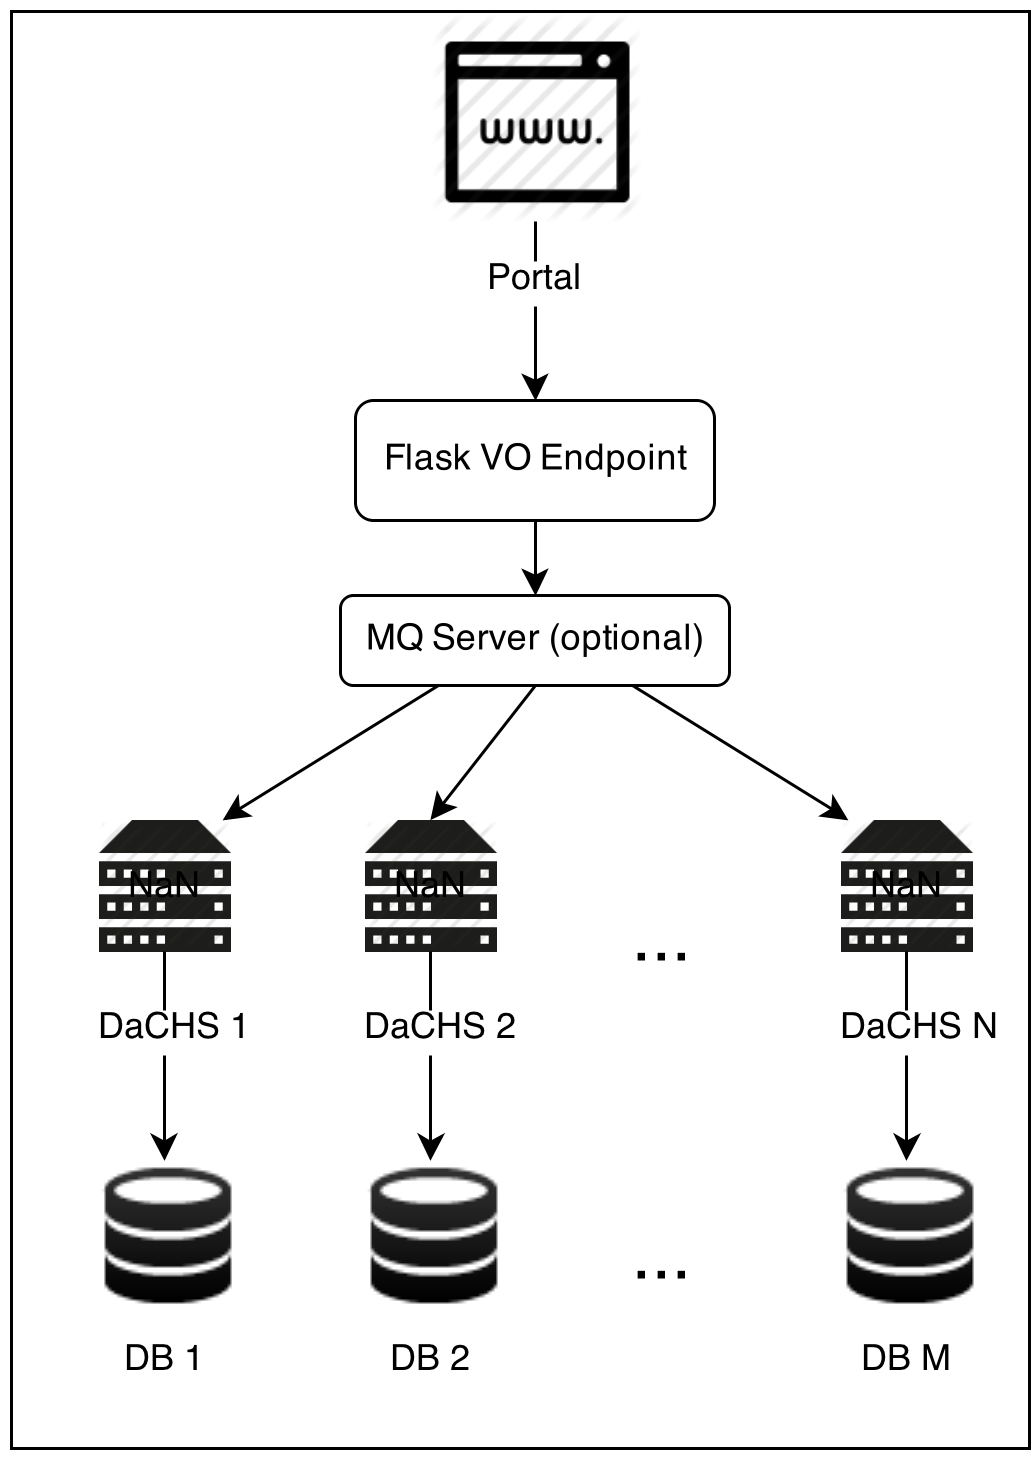
\includegraphics[width=0.4\textwidth]{img/interaccion.png}
        \caption{Arquitectura ChiVO - Interacción del servicio.}
    \end{center}
\end{figure}
